\documentclass[11pts,french]{article}

\usepackage[utf8]{inputenc}
\usepackage[left=1.5cm, right=1.5cm, top=1.5cm, bottom=1.5cm]{geometry}
\usepackage{amsmath}
\usepackage{caption}
\usepackage{tikz-qtree}
\usepackage{hyperref}
\usepackage[justification=centering]{caption}

\setlength{\parindent}{0pt}
\setlength{\textfloatsep}{5pt}
\setlength{\intextsep}{5pt}
\hypersetup{
    colorlinks=true,
    linkcolor=red,
    filecolor=magenta,
    citecolor=blue
    urlcolor=blue,
    pdftitle={Overleaf Example},
    pdfpagemode=FullScreen,
}

\newcommand{\acom}[1]{{\color{violet}(#1)}}
\newcommand{\okcom}[1]{{\color{blue}#1}}

\graphicspath{ {./images/} }

\title{Simulation par HPC de dynamique causal de graphe quantique}
\author{ Joseph TOUZET \\
encadré par Pablo ARRIGHI et Oguz KAYA \\
laboratoires LMF et LISN}
\date{Juin 2021}

\begin{document}

\maketitle

\abstract{
La physique quantique permet d'étudier des superpositions d'objets, et de prédire l'évolution de ces superpositions. En plus d'étudier une superposition de particules, on peut aussi étudier une superposition de l'espace sur lequel se trouve ces particules. \\

Cet espace sera ici un graphe circulaire, et les dynamiques étudiées pourront créer et détruire des noeuds. Ce modèle peut modéliser une dilatation ou contraction de l'espace, qui serait quantifiée.

Nous chercherons à : avoir une implémentation efficace de ce modèle (parallélisme, calcul distribué, etc...) car la complexité de la simulation quantique est d'ordre exponentiel (car le nombre de graphes croit de manière exponentielle); concevoir une dynamique causant une croissance exponentielle de la taille moyenne des graphes, qui serait un modèle jouet de l'inflation pour un espace quantifié. 
}

\pagebreak{}

\section{Introduction}

Les graphes que nous étudions dans ce modèle jouet sont des cycles, où des particules peuvent se trouver ou non dans deux positions par noeud: le "port gauche" et le "port droit" qui dans l'étape de pas correspondent aux particules qui se déplacent respectivement vers la gauche et vers la droite.

\begin{figure}[ht]
\centering
\begin{minipage}{0.47\textwidth}
\raggedleft
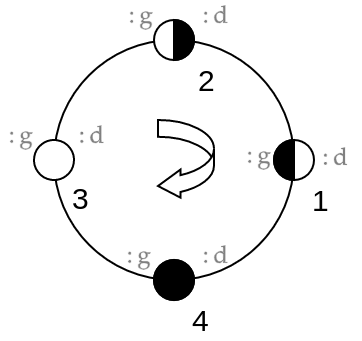
\includegraphics[width=3cm]{introduction}
\end{minipage}
\hspace{\fill} % note: no blank line here
\begin{minipage}{0.47\textwidth}
\caption{Exemple de graphe\\
1: Une particule au port gauche\\
2: Une particule au port droit\\
3: Noeud sans particule\\
4: Une particule sur chaque port}
\end{minipage}
\end{figure}

On peut ensuite appliquer à ces graphes des dynamique qui déterminent le futur état d'un noeud du graphe à partir de son état et de l'état de ses voisins. Une dynamique peut aussi créer ou détruire des noeuds et particules. \\

Il est intéressant de noter qu'une dynamique réversible peut causer une croissance du nombre de noeuds \cite{meyer1}. Nous nous posons donc la question de cette variation du nombre de noeuds si nous appliquons cette dynamique de manière analogue à une marche quantique \cite{meyer2}. Est-il alors possible d'observer une croissance qui ne suit pas la courbe moyenne classique ? \\

Pour répondre à ces questions il est important d'avoir une implémention de ce modèle extrêmement efficace, dont la programmation est le sujet de mon stage.

\section{ Dynamique classique }

Les dynamiques que nous étudierons peuvent être représentées par un ensemble de 2 motifs locaux qui sont échangés par la dynamique.

\begin{figure}[ht]
\begin{minipage}{0.50\textwidth}
\centering
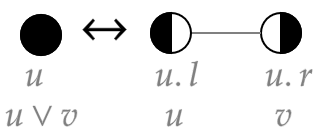
\includegraphics[width=3cm]{split_merge}
\caption{motifs échangés par SM}
\end{minipage}
\begin{minipage}{0.50\textwidth}
\vspace*{0.4cm}
\centering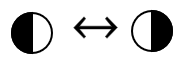
\includegraphics[width=2cm]{coin}
\vspace*{0.2cm}
\caption{motifs échangés par la dynamique coin}
\end{minipage}


\vspace*{0cm} % vertical separation

\begin{minipage}{0.40\textwidth}
\centering
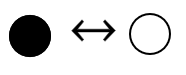
\includegraphics[width=2cm]{erase_create}
\caption{motifs échangés par EC}
\end{minipage}
\begin{minipage}{0.60\textwidth}
\centering
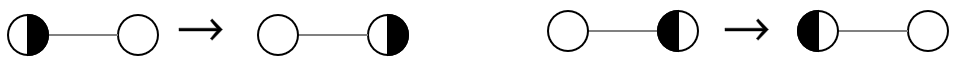
\includegraphics[width=10cm]{move}
\caption{motifs échangé par M}
\end{minipage}

\captionsetup{labelformat=empty}
\caption{motifs échangés par les différentes dynamiques}

\end{figure}

Les différentes dynamiques étudiées jusqu'ici sont:

\begin{itemize}
\itemsep0em
    \item La dynamique "erase create" (notée EC) permet la création de particules, mais ne "merge" ou "split" pas de noeuds.
    
    \item La dynamique "split merge" (notée SM) permet la création (par "split") et la destruction (par "merge") de noeuds, mais conserve le nombre de particules.
    
    \item L'étape de pas (notée M et qui sera toujours classique) fais simplement bouger les particules dans le port gauche d'un noeud vers le port gauche du noeud à leur gauche, et inversement pour les particules allant à droite. Cette dynamique peut être très simplement inversé en déplaçant les particules à droite vers la gauche et inversement.
    
    \item La dynamique coin est une dynamique qui permet une marche quantique en faisant changer de direction une particule.
\end{itemize}

\subsection{ Arithmétique de nom }
\label{ssec:arbre}

Il est nécessaire de nommer les noeuds \cite{noms1} pour conserver la réversibilité \cite{noms2}. Cette condition nous donne aussi :

\begin{itemize}
\itemsep0em
    \item $\left(u \vee v\right).l = u$
    \item $\left(u \vee v\right).r = v$
    \item $u.r \vee u.l = u$
\end{itemize}

En prenant comme noms de départ des entiers naturels, on peut représenter les noms de noeud comme des arbres, par exemple:\\

\hfil
\Tree [ .{$\left( 0.r \vee 1 \right) \vee 2.l$}
[ .{$0.r \vee 1$}
[ .{$0.r$}
0
{$.r$} ]
1 ]
[ .{$2.l$}
2
{$.l$} ] ]

\section{ Dynamique quantique }

\subsection{ Paramétrisation }

Pour quantifier la dynamique, on rend l'échange de motif sujet à une opération unitaire paramétrée par 2 angles réels :

$$
U = \begin{pmatrix}
cos \theta & sin \theta e^{i\phi}\\ 
sin \theta e^{-i\phi} & -cos \theta
\end{pmatrix}
$$

En effet, en se plaçant dans la base "locale" (celle des deux motifs échangés par la dynamique), on décrit les amplitudes caractéristiques de la dynamique comme étant:

\begin{itemize}
\itemsep0em
    \item $sin \theta e^{i\phi} $ pour l'application dans le sens direct.
    \item $cos \theta $ pour la non-application dans le sens direct.
    \item $sin \theta e^{-i\phi} $ pour l'application dans le sens contraire.
    \item $cos \theta $ pour la non-application dans le sens contraire.
\end{itemize}

On remarque que l'angle $\phi$ peut favoriser ou non les interférences destructives ou constructives en influençant la phase relative de graphes ayant eu un différent nombre d'opération. \\

L'angle $\theta$ influence quant à lui la probabilité d'application par rapport à la probabilité de non-application. On a donc la dynamique classique pour $\theta = \frac{\pi}{2}$, on a aucun changement d'une itération à l'autre pour $\theta = 0$, et des dynamique intermédiaire pour $\theta$ entre $0$ et $\frac{\pi}{2}$.

\section{ Implémentation }

L'implémentation que j'ai codé lors de ce stage est codé en C++, en reposant sur OpenMP pour le parallélisme et la bibliothèque \href{http://www.mpfr.org}{MPFR} pour permettre une plus grande précision de flottants dont nous avons besoin dans le calcul des probabilités.

\subsection{ Difficultés }

Le nom des noeuds doit être représenté par un arbre binaire (cf section \ref{ssec:arbre}), ce qui est une structure de donnée irrégulière et peut donc facilement limiter la vitesses d'accès mémoire en causant de la fragmentation en fonction des implémentions et de leur flexibilité. \\

On a une croissance exponentielle du nombre de graphes puisque chaque graphe tend à avoir un nombre constant en moyenne de sous-graphes engendrés après une étape de dynamique quantique. Ce qui nous condamne à être limités en mémoire après un faible nombre d'itérations.  \\

De plus chaque graphes est un relativement petit objet, et en créer et en détruire en permanence force un grand nombre d'allocations et de désallocations de petits objets, ce qui peut être très coûteux. \\

La dynamique quantique crée des graphes identiques qui doivent interférer (leurs amplitudes doivent être sommées) ce qui nous force à opérer un grand nombre de comparaisons d'objets irréguliers.

\subsection{ Techniques utilisé }

Nous représentons les noms de noeuds de manière continue en mémoire en utilisant des vecteurs d'indices à gauche et à droite plutôt que des containers. Ce qui nous force à prévoir le nombre maximal de noeuds dans ces arbres avant de créer les graphes.  \\

De plus, chaque propriété, relatives aux graphes individuels, aux noeuds ou aux arbre de noeud, est représentée sous la forme d'un seul vecteur contig\"u (que l'on ne fait qu'agrandir si besoin, sans jamais le rétrécir, et en s'interdisant les insertions et les suppressions). On se limite donc à un faible nombre, constant (autour d'un vingtaine), de grands objet contig\"us, ce qui permet de meilleurs accès mémoire en évitant la fragmentation. \\

Pour limiter la croissance exponentielle, nous gardons les $N$ graphes les plus probables après chaque itération. Nous prenons $N$ le plus grand possible sans pour autant remplir l'entièreté de la mémoire disponible ($N$ est de l'ordre de $10^{7}$ pour une machine avec 128Go de mémoire et pour des graphes de $10$ noeud de départ). \\

Pour pouvoir garder une représentation continue en mémoire de tout nos objets, et pour simplifier les interférences on commence par une itération symbolique où:

\begin{itemize}
\itemsep0em
    \item On calcule la taille de chaque objet à la prochaine itération pour pouvoir assigner des espaces mémoire continus (sur les vecteurs décris précédemment) pour chacun d'entre eux ce qui permettra leur accès en parallèle sans risque de ré-allocation.
    \item On calcule un hash de chaque graphe, pour ensuite effectuer l'interférence en les comparant plutôt que de comparer les graphes. On peut ensuite s'assurer de ne générer que des graphes distincts puisque l'interférence se fait à l'itération symbolique plutôt qu'à l'itération finale.
\end{itemize}

Ces techniques nous permettent d'avoir un fort gain de performance avec le nombre de coeurs (gain quasi-linéaire jusqu'à 8 coeur avant d'être limité par la bande passante de la mémoire, et arriver à un gain de 20x pour 32 coeurs).

\section{ Résultats }

\subsection{ Test et validation }

Le test le plus important d'une dynamique quantique est sa réversibilité: on veut s'assurer que après N étapes, on récupère bien l'état de départ avec une probabilité 1 en effectuant N étapes de la dynamique inverse. \\

Sachant que $EC \circ EC = I$ et $SM \circ SM = I$, et en notant $M^{-1}$ tel que $M \circ M^{-1} = I$, on peut trouver simplement l'inverse de règles composé simple:

\begin{itemize}
\itemsep0em
  \item $\left(EC \circ M\right)^{-1} = M^{-1} \circ EC$
  \item $\left(SM \circ M\right)^{-1} = M^{-1} \circ SM$
\end{itemize}

On peut ensuite opérer ce test d'objectivité pour des milliers de graphes aléatoires de tailles différentes, pour des valeurs de N différentes, et pour chacune de ces dynamiques. Permettant ainsi à la fois de vérifier la validité de chaque dynamique mais aussi la validité de l'implémention de l'application d'une dynamique quantique.

\subsection{ Simulation quantiques }

Nous calculons la taille moyenne et le nombre de particules moyen pour un certain nombre d'itérations de chaque règle, et la probabilité totale (pour mesurer l'impact de la suppression de graphes), le nombre de graphes et le ratio du nombre de graphes avant et après interférence. \\

\begin{figure}[h!]
\begin{minipage}{0.33\textwidth}
\centering
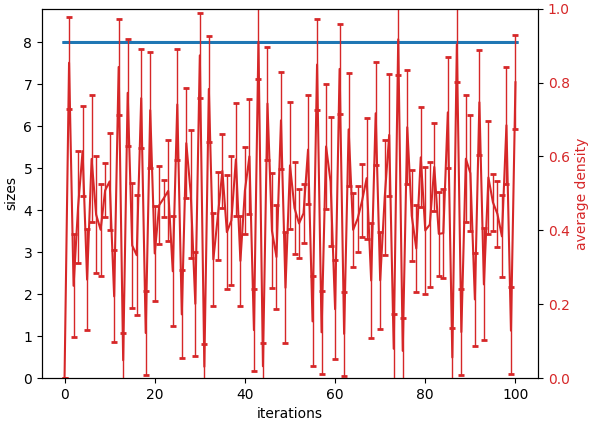
\includegraphics[width=\textwidth, height=0.66\textwidth]{sizes/0_erase_create_move}
\caption{$EC\circ M$, $\theta=0.375\pi$}
\end{minipage}
\begin{minipage}{0.33\textwidth}
\centering
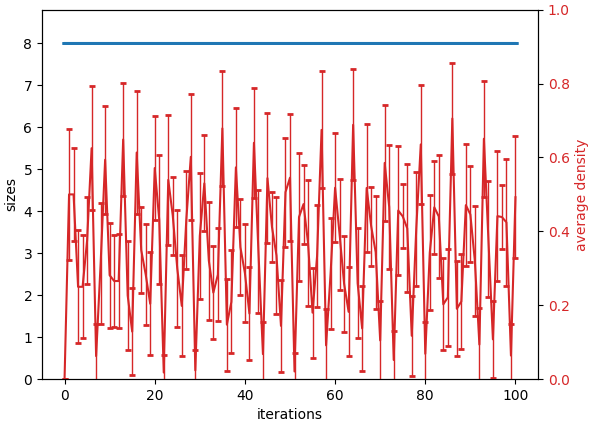
\includegraphics[width=\textwidth, height=0.66\textwidth]{sizes/2_erase_create_move}
\caption{$EC\circ M$, $\theta=0.25\pi$}
\end{minipage}
\begin{minipage}{0.33\textwidth}
\centering
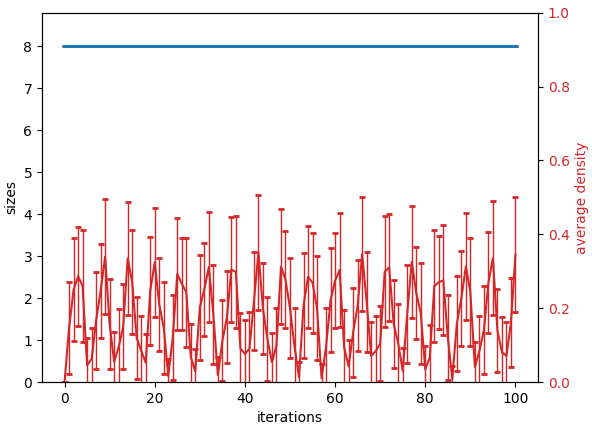
\includegraphics[width=\textwidth, height=0.66\textwidth]{sizes/1_erase_create_move}
\caption{$EC\circ M$, $\theta=0.125\pi$}
\end{minipage}

\captionsetup{labelformat=empty}
\caption{Bleu foncé: probabilité total, Rouge: nombre de graphes (échelle log.), bleu clair: ratio du nombre de graphes avant/après interférence }

\end{figure}

On remarque que pour la dynamique $EC \circ M$ (figures 7 à 9, en partant d'un graphe vide) la densité de particules oscille avec une amplitude dépendante de $\theta$ (plus $\theta$ est grand plus la probabilité d'opération est grande, ce qui créer des particules à l'itération N et les détruit à l'itération N-1). \\

\begin{figure}[h!]
\begin{minipage}{0.33\textwidth}
\centering
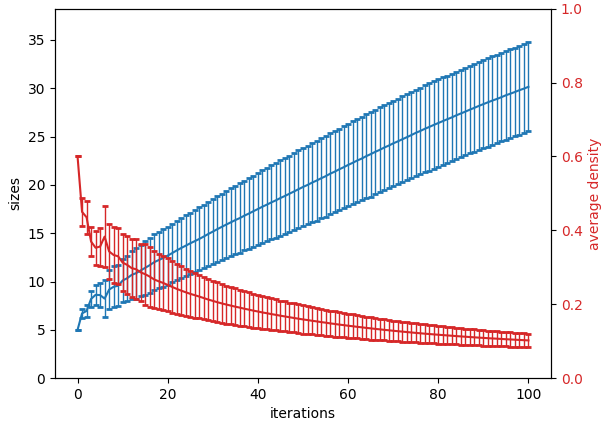
\includegraphics[width=\textwidth, height=0.66\textwidth]{sizes/0_split_merge_move}
\caption{$SM\circ M$, $\theta=0.375\pi$}
\end{minipage}
\begin{minipage}{0.33\textwidth}
\centering
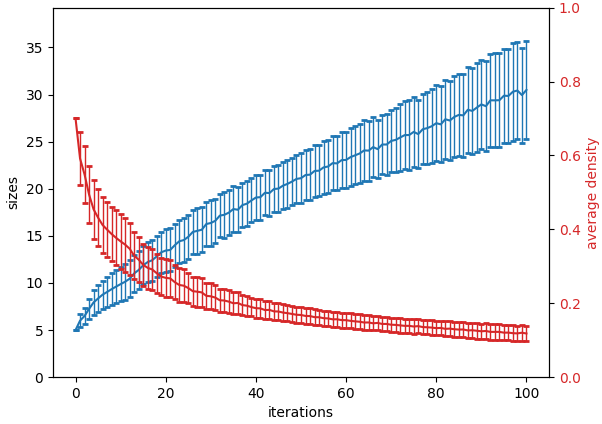
\includegraphics[width=\textwidth, height=0.66\textwidth]{sizes/1_split_merge_move}
\caption{$SM\circ M$, $\theta=0.25\pi$}
\end{minipage}
\begin{minipage}{0.33\textwidth}
\centering
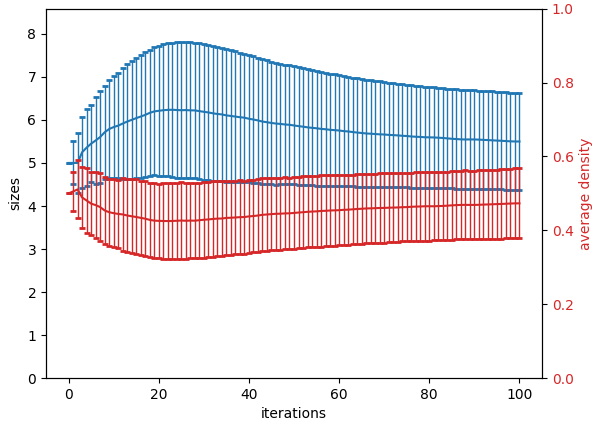
\includegraphics[width=\textwidth, height=0.66\textwidth]{sizes/2_split_merge_move}
\caption{$SM\circ M$, $\theta=0.125\pi$}
\end{minipage}

\captionsetup{labelformat=empty}
\caption{Bleu: taille moyenne, Rouge: densité moyenne}

\end{figure}

Pour la dynamique $SM \circ M$ (figures 11 à 13) la taille moyenne croît de manière classique (la densité décroît inversement au nombre de noeuds puisque le nombre de particules est constant) pour $\theta \neq 0.25\pi$ mais avec une croissance plus faible pour $\theta$ plus faible. \\

Pour $\theta = 0.125\pi$ On a d'abord une croissance, puis une décroissance lorsque le nombre de graphes explose et que les graphes ayant beaucoup de "split merge" (et donc les plus grand) deviennent exponentiellement moins probables par rapport aux graphes restés de taille constante. Il n'est pas clair si se résultat est uniquement du à la suppression des graphes les moins probables ou non. \\

\begin{figure}[h!]
\begin{minipage}{0.33\textwidth}
\centering
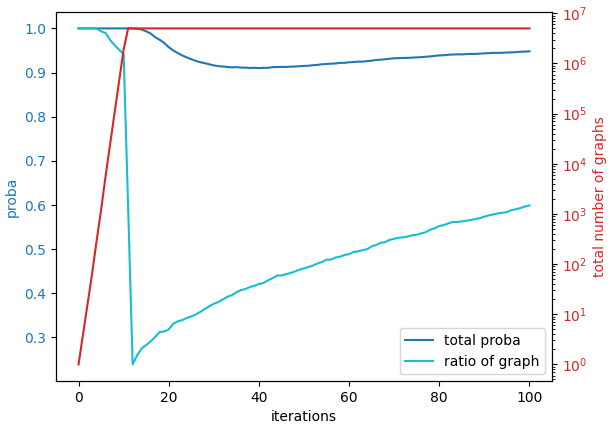
\includegraphics[width=\textwidth, height=0.66\textwidth]{stats/0_split_merge_move}
\caption{$SM\circ M$, $\theta=0.375\pi$}
\end{minipage}
\begin{minipage}{0.33\textwidth}
\centering
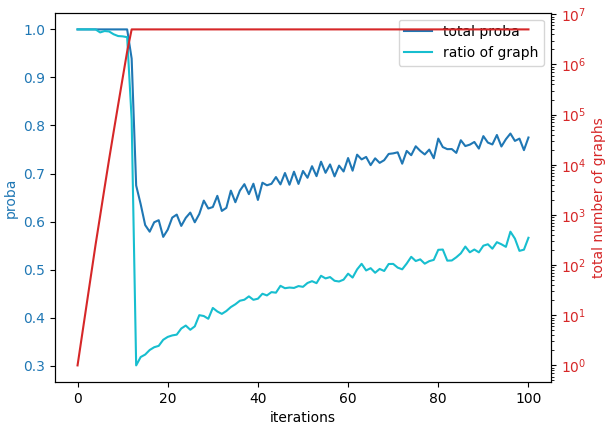
\includegraphics[width=\textwidth, height=0.66\textwidth]{stats/1_split_merge_move}
\caption{$SM\circ M$, $\theta=0.25\pi$}
\end{minipage}
\begin{minipage}{0.33\textwidth}
\centering
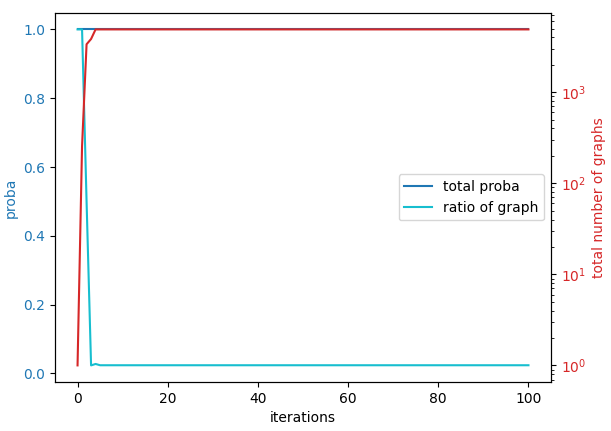
\includegraphics[width=\textwidth, height=0.66\textwidth]{stats/2_erase_create_move}
\caption{$EC\circ M$, $\theta=0.25\pi$}
\end{minipage}

\captionsetup{labelformat=empty}
\caption{Bleu foncé: probabilité total, Rouge: nombre de graphes (échelle log.), bleu clair: ratio du nombre de graphes avant/après interférence }

\end{figure}

Les instabilités pour la dynamique $SM \circ M$ et $\theta=0.25\pi$ sont expliquées par la figure 16: on peut voir que l'on a une forte perte de probabilité totale, qui est due à une trop faible variation de probabilité des graphe (car $\theta=0.25\pi$) ce qui amène à avoir une perte de probabilité quasi-égale à la proportion de graphe supprimé. \\

On remarque aussi que la croissance du nombre de graphes est très exactement exponentielle (droite en échelle log), et que la dynamique $EC \circ M$ (figure 17) a un comportement typiquement quantique puisque son ratio de graphes est proche de zéro (très grand nombre de graphes qui interagissent) car elle est limité en nombre de graphes par $4^n$ avec n le nombre de noeuds.

\section{ Suite du stage }

Maintenant que l'on a la capacité de faire une simulation quantique, les objectifs pour les 4 prochaine semaine de stage sont:

\begin{itemize}
\itemsep0em
    \item Concevoir une dynamique qui cause une croissance exponentielle du nombre de noeuds.
    \item Observer des comportement typiquement quantique (distinct du comportement probabiliste, et dépendant de l'angle $\phi$).
    \item Observer les limites des approximations faites.
\end{itemize}

\pagebreak{}

\section{ Conclusion }

Les techniques de simulation et programmation, et les approximations utilisées jusqu'ici ont permis d'obtenir des résultat de simulation pour un problème qui, sans approximation est de complexité au moins exponentielle (avec le nombre de graphes). On peut maintenant espérer concevoir une dynamique causant une croissance exponentielle de la taille, bien que certain résultat préliminaires montrent que cette dynamique peut être plus complexe qu'il n'y parait (non-stabilité de la densité avec la règle $EC \circ M$, et une observation récente que une dynamique $EC \circ M \circ SM \circ M$ ou $EC \circ SM \circ M$ a tendance à revenir à l'état de départ et donc à empêcher la croissance). \\

Ce stage est ma première expérience de programmation pour la recherche. C'est aussi la première fois que j'ai eu l'occasion d'utiliser des machines si puissantes, ce qui amène des considération d'HPC que je n'ai jamais eues, et m'a permis de prendre en considération des aspects d'optimisation très enrichissants.

\vfill
\bibliographystyle{abbrv}
\bibliography{biblio}

\end{document}
